\documentclass[english,12pt,a4paper]{report}
\usepackage[T1]{fontenc}
\usepackage{babel}
\usepackage{geometry}
\geometry{
	a4paper,
	total={170mm,257mm},
	left=20mm,
	top=20mm,
}
\usepackage{easyReview}
\usepackage{hyperref}
\hypersetup{
	hidelinks=true,
	colorlinks=true,
	linkcolor=black,
	filecolor=magenta,      
	urlcolor=blue,
	pdftitle={Final Project},
	pdfpagemode=FullScreen,
}
\usepackage{amsmath}
\usepackage{pgfplots}
\usepackage{xcolor}
\usepackage{listings}
\lstdefinestyle{mystyle}{
	commentstyle=\color{green},
	keywordstyle=\color{blue},
%	numberstyle=\tiny\color{codegray},
	stringstyle=\color{magenta},
	basicstyle=\ttfamily\footnotesize,
	breakatwhitespace=false,         
	breaklines=true,                 
	captionpos=t,                    
	keepspaces=true,
	tabsize=2,
	prebreak=\raisebox{0ex}[0ex][0ex]{\ensuremath{\hookleftarrow}}
}

\lstset{style=mystyle}


% Computation of Trajectory in Two-Body Problem
% Numerical Solution of Two-Body Problem
\title{Numerical Methods for Solving Ordinary Differential Equations in Two-Body Problem\\
	\normalsize Computation Techniques Final Project}

\author{Kamil Chaj}



\date{2023/2024}
\begin{document}
	\begin{titlepage}
		\noindent
		Supervised by: Przemysław Korohoda, Dr. Eng \\
		Date of submission: DD/MM/YYYY
		\begin{center}

			\vspace*{-1cm}

			\vfill
			
			\textbf{Numerical Methods for Solving Differential Equations in Two-Body Problem}
						
			\vspace{0.5cm}
			
			\textit{Computation Techniques Final Project}
			
			\vspace{1.5cm}
			
			Kamil Chaj
			
			\vspace{1.5cm}
			
%			Supervised by: Przemysław Korohoda, Dr. Eng \\
%			Date of submission: DD/MM/YYYY
			
			\vfill
									
			Computational Techniques \\
			Electronics and Telecommunications \\
			AGH University of Science and Technology, Kraków, Poland\\
			2023/2024
			
		\end{center}
	\end{titlepage}
	\begin{abstract}
		Two-body problem discuss predicting orbit of two bodies viewed as point masses. The problem assumes that the two objects interact only with one another, and all other bodies are ignored. Goal of this project is to implement and test different methods of numerically solving ordinary differential equations in case of two-body problem. Methods we are going to implement and compare are matrix system of first order differential equations, Euler method, Runge-Kutta method and build-in ODE solvers in MATLAB. 
		
		(brief summery of results ...)
	\end{abstract}
		\tableofcontents
	\chapter{Two Body Problem}
	\section{Assumptions}
	For the problem to be not too complicated we can take few assumptions that will simplify solution but maintain overall correct results.
	
	\begin{itemize}
		\item in system there exists only two bodies
		%				\item \alert{One of the bodies is significantly smaller and less massive then the other}
		\item bodies have uniform mass distributions and are perfectly symmetrical
		%				\item distance between surfaces of bodies is much greater then radius of smaller body
		%				\item reference frame is inertial and centered at central body geometric center
	\end{itemize}
	
	\section{Two-body system}
	
	In the system we define two bodies with masses $m_1$, $m_2$ and positions $\vec{r_1}$, $\vec{r_2}$, where distance between bodies is represented by $\vec{r_0}$ which can be described by following equation.
	
	\begin{equation}\label{vec}
		\vec{r_0} = \vec{r_2} - \vec{r_1}
	\end{equation}
	
	\begin{figure}[h!]
		\begin{center}
			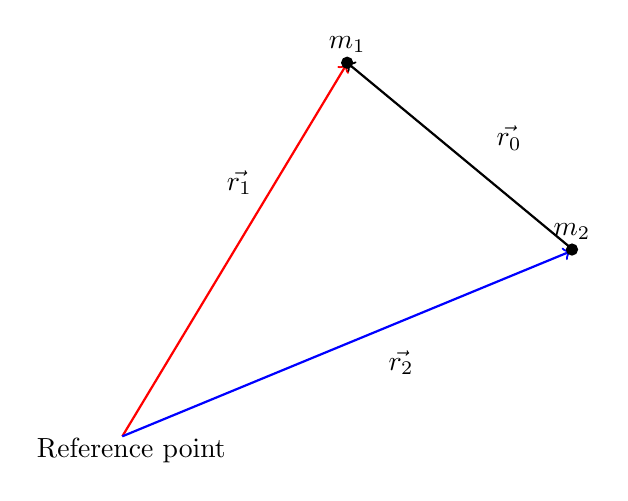
\begin{tikzpicture}
				\begin{axis}[
					hide axis,
					clip=false
					]
					\addplot[
					->, thick, red
					] coordinates {
						(0, 0) (2.99, 1.99) 
					};
					\addplot[
					->, thick, blue
					] coordinates {
						(0, 0) (5.98, 0.99)
					};
					\addplot[
					->, thick
					] coordinates {
						(5.98, 1.01) (3, 2) 
					};
					\node[above] at  (axis description cs:0.8,0.7) {$\vec{r_0}$};
					\node[above] at  (axis description cs:0.3,0.6) {$\vec{r_1}$};
					\node[above] at  (axis description cs:0.6,0.2) {$\vec{r_2}$};
					\node[below] at  (axis description cs:0.1,0.1) {Reference point};
					
					\addplot [mark=*,nodes near coords,only marks,point meta=explicit symbolic]
					table[meta=label] {
						x   y   label
						3   2   $m_1$
						6   1	$m_2$
					};					
				\end{axis}
			\end{tikzpicture}
		\end{center}
		\caption{two-body system}
	\end{figure}	
	
	\section{Derivation of differential equation}
	
	Lets start derivation with defining forces $\vec{F_{12}}$ and $\vec{F_{21}}$ and relation between these forces coming from our assumption that there are only two bodies and therefore only two forces which net force is zero.
		
	\begin{equation}\label{ef1}
		m_1 \frac{d^2\vec{r_1}}{dt^2} = \vec{F_{12}}
	\end{equation}
	\begin{equation}\label{ef2}
		m_2 \frac{d^2\vec{r_2}}{dt^2} = \vec{F_{21}}
	\end{equation}
	\begin{equation}\label{ef3}
		\vec{F_{12}} = - \vec{F_{21}} = \vec{F}
	\end{equation}
	
	After combining above equations we get system of differential equation describing behavior of any two-body system.
	
	\begin{equation}\label{gen_tb}
		\begin{cases}
			m_1 \frac{d^2\vec{r_1}}{dt^2} = \vec{F} \\
			m_2 \frac{d^2\vec{r_2}}{dt^2} = - \vec{F} \\
		\end{cases}
	\end{equation}
	
	
	\section{System of two planets}
	In our case we want to investigate two-body system where force $\vec{F}$ is described by Newton's law of universal gravitation (\ref{uni_newton})
	\begin{equation}\label{uni_newton}
		\vec{F} = G \frac{m_1 m_2}{r_0^2}\hat{r_0}, \qquad \hat{r_0} = \frac{\vec{r_0}}{r_0}
	\end{equation}
	By substituting $\vec{F}$ (\ref{uni_newton}) and $\vec{r_0}$ (\ref{vec}) in equation (\ref{gen_tb}) we get final system of nonlinear differential equations.
	\begin{equation}
		\begin{cases}
			\dfrac{d^2\vec{r_1}}{dt^2} =  \dfrac{G m_2}{||\vec{r_2} - \vec{r_1}||^3} (\vec{r_2} - \vec{r_1})\\
			\dfrac{d^2\vec{r_2}}{dt^2} =  \dfrac{G m_1}{||\vec{r_2} - \vec{r_1}||^3} (\vec{r_1} - \vec{r_2})
		\end{cases}
	\end{equation}	
	
	\section{Initial conditions}
	
	For second order differential equation we need to specify position and velocity at some time, usually at time = 0, to find particular solution. In our system we have two second order equation therefore we need two initial position and velocity vectors which gives us 12 scalar quantities if we consider three dimensional case.
	
	\begin{equation}
		\begin{bmatrix}
			\vec{r_1}(t_0) \\ \vec{r_2}(t_0) \\ \vec{v_1}(t_0) \\ \vec{v_2}(t_0)
		\end{bmatrix}
		=
		\begin{bmatrix}
			x_1(t_0) & y_1(t_0) & z_1(t_0)\\
			x_2(t_0) & y_2(t_0) & z_2(t_0)\\
			v_{x1}(t_0) & v_{y1}(t_0) & v_{z1}(t_0)\\
			v_{x1}(t_0) & v_{y1}(t_0) & v_{z1}(t_0)
		\end{bmatrix}
		, \qquad t_0 = 0
	\end{equation}
	
	\subsection{Earth-Moon system}
	
	First we need to assign values for all parameters in our equations.
	$G$ parameter is Newtonian constant of gravitation, note that this constant dictates what unites we have to use later
	
	\begin{equation}\label{eq:G}
		G = 6.6743 \cdot 10^{-11} m^3 kg^{-1} s^{-2}
	\end{equation}
	
	Mass of the Earth
	$$ m_1 = 5.97 \cdot 10^{24} kg $$
	
	Mass of the Moon
	$$ m_2 = 7.34 \cdot 10^{22} kg $$
	
	And initial conditions for the system, $\vec{v_{moon}}$ is perpendicular to position vector, $v_{earth}$ is velocity of Earth and Moon around Sun
	$$
	v_{moon} = 1.022 \cdot 10^3 \frac{m}{s}
	, \qquad v_{earth} = 29.78 \cdot 10^3 \frac{m}{s}
	, \qquad r_0 = 3.844 \cdot 10^5 km
	$$
	
	\begin{equation}
%		\begin{split}
%			\vec{r_1}(0) &= 
%			\begin{bmatrix}
%				0 & 0 & 0
%			\end{bmatrix} \\
%			\vec{v_1}(0) &= 
%			\begin{bmatrix}
%				0 & 0 & v_{earth}
%			\end{bmatrix} \\ 
%			\vec{r_2}(0) &= 
%			\begin{bmatrix}
%				r_0 & 0 & 0
%			\end{bmatrix} \\
%			\vec{v_2}(0) &= 
%			\begin{bmatrix}
%				0 & v_{moon} & v_{earth}
%			\end{bmatrix}
%		\end{split}
		\begin{bmatrix}
			\vec{v_1}(0)\\
			\vec{v_2}(0)\\
			\vec{r_1}(0)\\
			\vec{r_2}(0)\\
		\end{bmatrix}
		=
		\begin{bmatrix}
			0 & v_{moon} & v_{earth}\\
			0 & 0 & v_{earth}\\
			0 & 0 & 0\\
			r_0 & 0 & 0\\
		\end{bmatrix}
	\end{equation}
	
	\subsection{Equal masses system}
	
	Gravitation constant $G$ stays the same as in previous case (\ref{eq:G}). Both masses are equal and for this example we will use 2 Marses.
	
	$$ m_1 = m_2 = 0.641 \cdot 10^{24} kg $$
	
	Because it is purely hypothetical example we can set any initial values. 
	
	$$
	v_{1} = 1 \cdot 10^3 \frac{m}{s}
	, \qquad v_{2} = 1 \cdot 10^3 \frac{m}{s}
	, \qquad r_0 = 1 \cdot 10^{8} m
	$$
		
	\begin{equation}
%		\begin{split}
%			\vec{r_1}(0) &= 
%			\begin{bmatrix}
%				0 & 0 & 0
%			\end{bmatrix} \\
%			\vec{v_1}(0) &= 
%			\begin{bmatrix}
%				0 & v_1 & 0
%			\end{bmatrix} \\ 
%			\vec{r_2}(0) &= 
%			\begin{bmatrix}
%				r_0 & 0 & 0
%			\end{bmatrix} \\
%			\vec{v_2}(0) &= 
%			\begin{bmatrix}
%				0 & v_2 & 0
%			\end{bmatrix}
%		\end{split}
		\begin{bmatrix}
			\vec{v_1}(0)\\
			\vec{v_2}(0)\\
			\vec{r_1}(0)\\
			\vec{r_2}(0)\\
		\end{bmatrix}
		=
		\begin{bmatrix}
			0 & v_1 & 0\\
			0 & v_2 & 0\\
			0 & 0 & 0\\
			r_0 & 0 & 0\\
		\end{bmatrix}
	\end{equation}
	
	\subsection{Arbitrary system}
	
	\alert{IDK TBD}
	
	For this system we will start with general equation for two-body problem (\ref{gen_tb}) and specify Force with different expression which is linear.
	Force is proportional to distance between bodies
	
	\begin{equation}\label{gen_tb}
		\begin{cases}
			\frac{d^2\vec{r_1}}{dt^2} = \frac{\vec{r_2}-\vec{r_1}}{m_1} \\
			\frac{d^2\vec{r_2}}{dt^2} = \frac{\vec{r_2}+\vec{r_1}}{m_2} \\
		\end{cases}
	\end{equation}
	
		$$ m_1 = 10 kg$$
		
		$$ m_2 = 10 kg $$
	
	$$
	v_1 = 1 \frac{m}{s}
	, \qquad v_2 = 1 \frac{m}{s}
	, \qquad r_0 = 10 m
	$$
	
	\begin{equation}
		\begin{bmatrix}
			\vec{v_1}(0)\\
			\vec{v_2}(0)\\
			\vec{r_1}(0)\\
			\vec{r_2}(0)\\
		\end{bmatrix}
		=
		\begin{bmatrix}
			0 & v_1 & 0\\
			0 & -v_2 & 0\\
			-0.5r_0 & 0 & 0\\
			0.5r_0 & 0 & 0\\
		\end{bmatrix}
	\end{equation}
	
	\chapter{Numerical method for differential equations}
	
	In numerical approximations of differential equation we replace infinitesimal change $d$ with finite change $\Delta$ and iteratively calculate small pieces of the curve.
	
	\begin{equation}\label{eq:num}
		\frac{d \vec{v}}{dt} = f(\vec{r}, t) \implies \frac{\Delta \vec{v}}{\Delta t} = f(\vec{r}, t_n)
	\end{equation}
	
	\begin{equation}
		\begin{split}
			t_n &= t_0 + n \Delta t \\
			t_n &= t_{n-1} + \Delta t
		\end{split}
	\end{equation}
	
	By multiplying equation (\ref{eq:num}) by $\Delta t$ we get change of a function in time interval $\Delta t$
	
	\begin{equation}
		\Delta \vec{v} = f(\vec{r}, t_n) \Delta t
	\end{equation}
	
	Truncation error is cause by using finite time step and comes from the definition of limit. Truncation error can be used for adjusting time step in adaptive methods
	
	\begin{equation}
		\frac{\Delta \vec{v_{n+1}} - \Delta \vec{v_n}}{\Delta t} = \text{Truncation error}
	\end{equation}
	
	\section{Linear example}
	\alert{IDK TBD}
	
	Linear differential equations can be solved using method of undetermined coefficients
	
	\section{Euler method}
	This is the simplest method for solving differential equations, where next value is sum of current value and change evaluated at the beginning of $\Delta t$ 
		
	\begin{equation}
		\begin{split}
			\vec{r_{n+1}} &= \vec{r_{n}} + \Delta \vec{r} \\
			&= \vec{r_{n}} + f(\vec{r_n}, t_0 + n \Delta t) \Delta t
		\end{split}
	\end{equation}
	
	For higher order equations we simply need to convert n-th order equation to system of n first order equations
	
	\begin{equation}
		\begin{bmatrix}
			\vec{r_{n+1}}\\
			\vec{v_{n+1}}\\
		\end{bmatrix}
		=
		\begin{bmatrix}
			r_n + v_n \Delta t\\
			v_n + f(\vec{r_n}, t) \Delta t
		\end{bmatrix}
	\end{equation}
	
	\section{4th order Runge-Kutta method}
	
	Runge-Kutta method is similar to Euler method but instead of evaluating change of a function once per iteration, in case of 4th order method, it evaluates function 4 times per iteration, and takes weighted average of these evaluations.
	
	\begin{equation}
		\begin{split}
			k_1 &= f(\vec{r_n},  t_0 + n \Delta t)\\
			k_2 &= f\left(\vec{r_n} + k_1 \frac{\Delta t}{2}, t_0 + \Delta t(n + \frac{1}{2})\right)\\
			k_3 &= f\left(\vec{r_n} + k_2 \frac{\Delta t}{2}, t_0 + \Delta t(n + \frac{1}{2})\right)\\
			k_4 &= f\left(\vec{r_n} + k_3 \Delta t, t_0 + \Delta t(n + 1)\right)
		\end{split}
	\end{equation}
	
	Times at which each evaluation is calculated can be adjusted but the most common is to evaluated function once at beginning and end the interval and twice in the middle of the interval but for second evaluation taking result of the first as an input
	
	\begin{equation}
		\vec{v_{n+1}} = \vec{v_n} + \frac{\Delta t}{6}(k_1 + 2 k_2 + 2k_3 + k_4)
	\end{equation}
	
	Evaluation made in the middle of the interval have usually greater weight.	
	
	\begin{equation}
		\begin{bmatrix}
			\vec{r_{n+1}}\\
			\vec{v_{n+1}}\\
		\end{bmatrix}
		=
		\begin{bmatrix}
			r_n + v_n \Delta t\\
			v_n + \frac{\Delta t}{6}(k_1 + 2 k_2 + 2k_3 + k_4)
		\end{bmatrix}
	\end{equation}
	
	\section{Adaptive Runge-Kutta method}
	
	In adaptive Runge-Kutta method after each iteration program check if truncation does not exceed set limit, and if it does, evaluation is rejected and the same evaluation is made again with new time step calculated based on maximal and current error until truncation is within set error limit.
	
	For 4th order method new time step is calculated using following formula
	\begin{equation}
		\Delta \tau = \Delta t \left( \dfrac{\varepsilon}{e} \right) ^{\frac{1}{5}}
	\end{equation}
	$\Delta \tau$ - new time step, $e$ - truncation error, $\varepsilon$ - tolerance
	
	\section{Matlab ODE45 solver}
	
	\chapter{Results}
	
	\section{COOL PLOTS}
	
	\section{Accumulation error}
	
	\section{Computation time}
	
	\section{Conclusions}
	
	
	\appendix
	\chapter{Sources}
	\begin{enumerate}
		\item \href{https://nssdc.gsfc.nasa.gov/planetary/planetfact.html}{Planetary Fact Sheets - NASA}
		\item \href{https://www.youtube.com/playlist?list=PLkZjai-2Jcxn35XnijUtqqEg0Wi5Sn8ab}{Numerical Methods for Engineers - Jeffrey Chasnov}
		\item \href{https://www.youtube.com/playlist?list=PLOIRBaljOV8hBJS4m6brpmUrncqkyXBjB}{Fundamentals of Orbital Mechanics - Alfonso Gonzalez}
		\item Wikipedia
		\begin{enumerate}
			\item \href{https://en.wikipedia.org/wiki/Two-body_problem}{Two-body problem}
			\item \href{https://en.wikipedia.org/wiki/Newton%27s_law_of_universal_gravitation}{Newton's law of universal gravitation}
			\item \href{https://en.wikipedia.org/wiki/Runge%E2%80%93Kutta_methods}{Runge-Kutta methods}
			\item \href{https://en.wikipedia.org/wiki/Truncation_error_(numerical_integration)}{Truncation error}
		\end{enumerate}
		\item Fundamentals of Physics Extended 10th edition - Halliday \& Resnick
	\end{enumerate}
	\chapter{Code}
	Only core functions listed, all code is available on \href{https://github.com/kamilix2003/two-body}{Github repository}
	
	\lstinputlisting[language=matlab, caption={base\_ode.m}]{../matlab/base_ode.m}
	\lstinputlisting[language=matlab, caption={euler.m}]{../matlab/euler.m}
	\lstinputlisting[language=matlab, caption={RK4.m}]{../matlab/RK4.m}
	\lstinputlisting[language=matlab, caption={Adaptive\_RK.m}]{../matlab/Adaptive_RK.m}
	
\end{document}